\documentclass{article}\usepackage[]{graphicx}\usepackage[]{color}
%% maxwidth is the original width if it is less than linewidth
%% otherwise use linewidth (to make sure the graphics do not exceed the margin)
\makeatletter
\def\maxwidth{ %
  \ifdim\Gin@nat@width>\linewidth
    \linewidth
  \else
    \Gin@nat@width
  \fi
}
\makeatother

\definecolor{fgcolor}{rgb}{0.345, 0.345, 0.345}
\newcommand{\hlnum}[1]{\textcolor[rgb]{0.686,0.059,0.569}{#1}}%
\newcommand{\hlstr}[1]{\textcolor[rgb]{0.192,0.494,0.8}{#1}}%
\newcommand{\hlcom}[1]{\textcolor[rgb]{0.678,0.584,0.686}{\textit{#1}}}%
\newcommand{\hlopt}[1]{\textcolor[rgb]{0,0,0}{#1}}%
\newcommand{\hlstd}[1]{\textcolor[rgb]{0.345,0.345,0.345}{#1}}%
\newcommand{\hlkwa}[1]{\textcolor[rgb]{0.161,0.373,0.58}{\textbf{#1}}}%
\newcommand{\hlkwb}[1]{\textcolor[rgb]{0.69,0.353,0.396}{#1}}%
\newcommand{\hlkwc}[1]{\textcolor[rgb]{0.333,0.667,0.333}{#1}}%
\newcommand{\hlkwd}[1]{\textcolor[rgb]{0.737,0.353,0.396}{\textbf{#1}}}%

\usepackage{framed}
\makeatletter
\newenvironment{kframe}{%
 \def\at@end@of@kframe{}%
 \ifinner\ifhmode%
  \def\at@end@of@kframe{\end{minipage}}%
  \begin{minipage}{\columnwidth}%
 \fi\fi%
 \def\FrameCommand##1{\hskip\@totalleftmargin \hskip-\fboxsep
 \colorbox{shadecolor}{##1}\hskip-\fboxsep
     % There is no \\@totalrightmargin, so:
     \hskip-\linewidth \hskip-\@totalleftmargin \hskip\columnwidth}%
 \MakeFramed {\advance\hsize-\width
   \@totalleftmargin\z@ \linewidth\hsize
   \@setminipage}}%
 {\par\unskip\endMakeFramed%
 \at@end@of@kframe}
\makeatother

\definecolor{shadecolor}{rgb}{.97, .97, .97}
\definecolor{messagecolor}{rgb}{0, 0, 0}
\definecolor{warningcolor}{rgb}{1, 0, 1}
\definecolor{errorcolor}{rgb}{1, 0, 0}
\newenvironment{knitrout}{}{} % an empty environment to be redefined in TeX

\usepackage{alltt}
\usepackage{enumerate}
\usepackage{amsmath}
\IfFileExists{upquote.sty}{\usepackage{upquote}}{}
\begin{document}

\title{\huge \textbf{Stat 207 HW3} \\}
\author{\large Cheng Luo 912466499 \\ \large Fan Wu 912538518}
\maketitle

\clearpage

\section{26.4}

\begin{enumerate}[(a)]

\item

\begin{knitrout}
\definecolor{shadecolor}{rgb}{0.969, 0.969, 0.969}\color{fgcolor}\begin{kframe}
\begin{alltt}
  \hlstd{dat} \hlkwb{=} \hlkwd{read.table}\hlstd{(}\hlstr{"CH26PR04.txt"}\hlstd{)}
  \hlkwd{names}\hlstd{(dat)} \hlkwb{=} \hlkwd{c}\hlstd{(}\hlstr{"Y"}\hlstd{,} \hlstr{"A"}\hlstd{,} \hlstr{"B"}\hlstd{,} \hlstr{"k"}\hlstd{)}
  \hlstd{dat}\hlopt{$}\hlstd{A} \hlkwb{=} \hlkwd{factor}\hlstd{(dat}\hlopt{$}\hlstd{A)}
  \hlstd{dat}\hlopt{$}\hlstd{B} \hlkwb{=} \hlkwd{factor}\hlstd{(dat}\hlopt{$}\hlstd{B)}
  \hlstd{a} \hlkwb{=} \hlkwd{length}\hlstd{(}\hlkwd{unique}\hlstd{(dat}\hlopt{$}\hlstd{A))}
  \hlstd{b} \hlkwb{=} \hlkwd{length}\hlstd{(}\hlkwd{unique}\hlstd{(dat}\hlopt{$}\hlstd{B))}
  \hlstd{n} \hlkwb{=} \hlkwd{length}\hlstd{(}\hlkwd{unique}\hlstd{(dat}\hlopt{$}\hlstd{k))}
  \hlstd{model} \hlkwb{=} \hlkwd{aov}\hlstd{(Y} \hlopt{~} \hlstd{A} \hlopt{+} \hlstd{A}\hlopt{/}\hlstd{B,} \hlkwc{data} \hlstd{= dat)}
  \hlkwd{resid}\hlstd{(model)}
\end{alltt}
\begin{verbatim}
##    1    2    3    4    5    6    7    8    9   10   11   12   13   14   15 
##  3.2 -3.8  1.2 -4.8  4.2  0.2 -5.8  7.2 -3.8  2.2 -6.6  2.4 -4.6  7.4  1.4 
##   16   17   18   19   20   21   22   23   24   25   26   27   28   29   30 
## -7.6  3.4  1.4 -4.6  7.4 -1.8  5.2  0.2  4.2 -7.8 -6.2  0.8  4.8  2.8 -2.2 
##   31   32   33   34   35   36   37   38   39   40   41   42   43   44   45 
## -3.8  0.2  6.2  2.2 -4.8 -4.0  1.0  6.0 -2.0 -1.0 -7.8  6.2 -2.8  1.2  3.2 
##   46   47   48   49   50   51   52   53   54   55   56   57   58   59   60 
## -6.6  0.4  2.4 -1.6  5.4  6.6 -2.4 -1.4  1.6 -4.4 -6.4  5.6 -0.4  3.6 -2.4
\end{verbatim}
\begin{alltt}
  \hlkwd{par}\hlstd{(} \hlkwc{mfrow} \hlstd{=} \hlkwd{c}\hlstd{(}\hlnum{2}\hlstd{,}\hlnum{2}\hlstd{))}
  \hlkwd{plot}\hlstd{(model,} \hlkwc{which} \hlstd{=} \hlnum{1}\hlstd{)}
  \hlkwd{plot}\hlstd{(model,} \hlkwc{which} \hlstd{=} \hlnum{2}\hlstd{)}
\end{alltt}
\end{kframe}
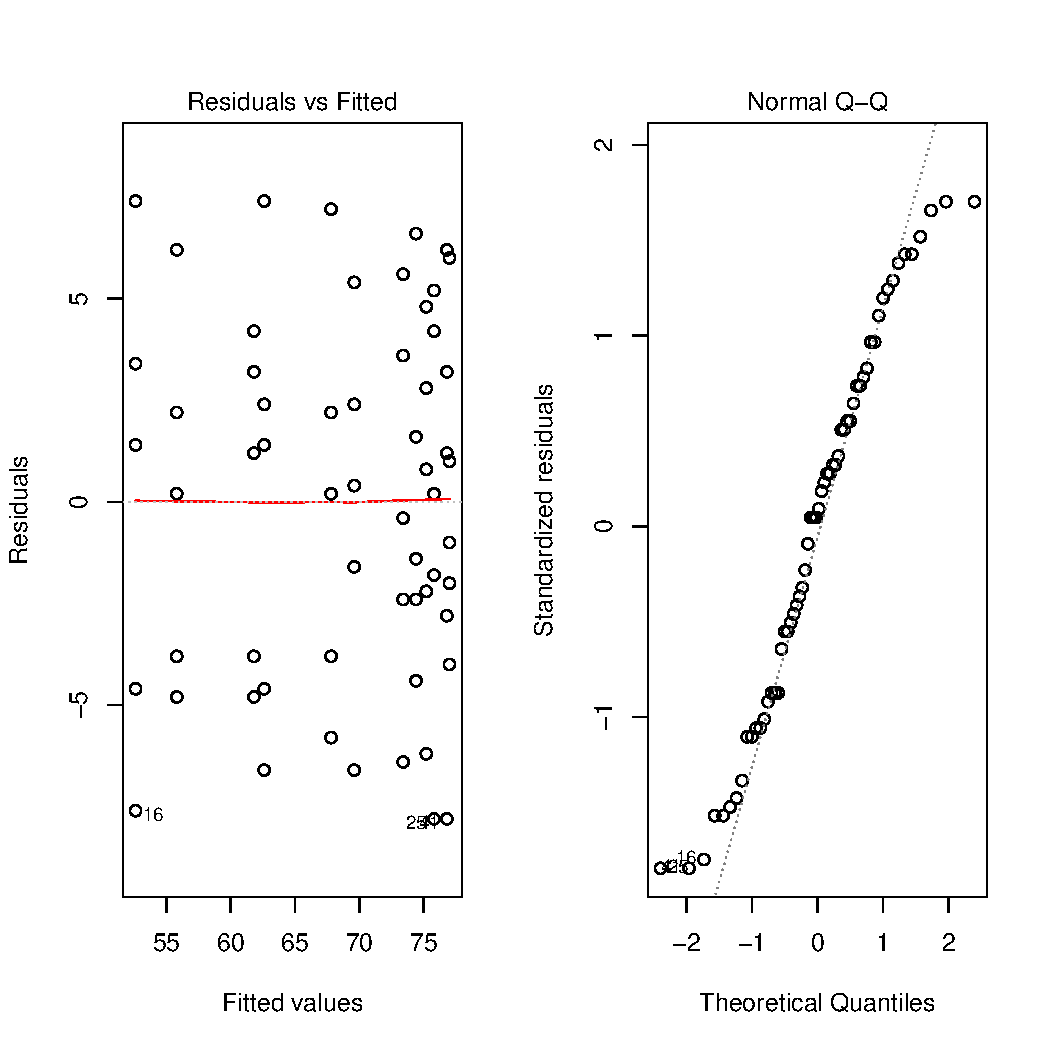
\includegraphics[width=\maxwidth]{figure/unnamed-chunk-1-1} 

\end{knitrout}

\qquad The residuals versus fitted values plots shows no sign for unequal variance.And the QQ-plot indicates approximately normal distribution with slightly light tail, so that normality assumption seems to be reasonable, we can use model(26.7) here.

\item

\begin{knitrout}
\definecolor{shadecolor}{rgb}{0.969, 0.969, 0.969}\color{fgcolor}\begin{kframe}
\begin{alltt}
  \hlkwd{require}\hlstd{(}\hlstr{"lattice"}\hlstd{)}
\end{alltt}


{\ttfamily\noindent\itshape\color{messagecolor}{\#\# Loading required package: lattice}}\begin{alltt}
  \hlkwd{dotplot}\hlstd{(}\hlkwd{resid}\hlstd{(model)} \hlopt{~} \hlstd{dat}\hlopt{$}\hlstd{A,} \hlkwc{xlab} \hlstd{=} \hlstr{"Machine"} \hlstd{)}
\end{alltt}
\end{kframe}
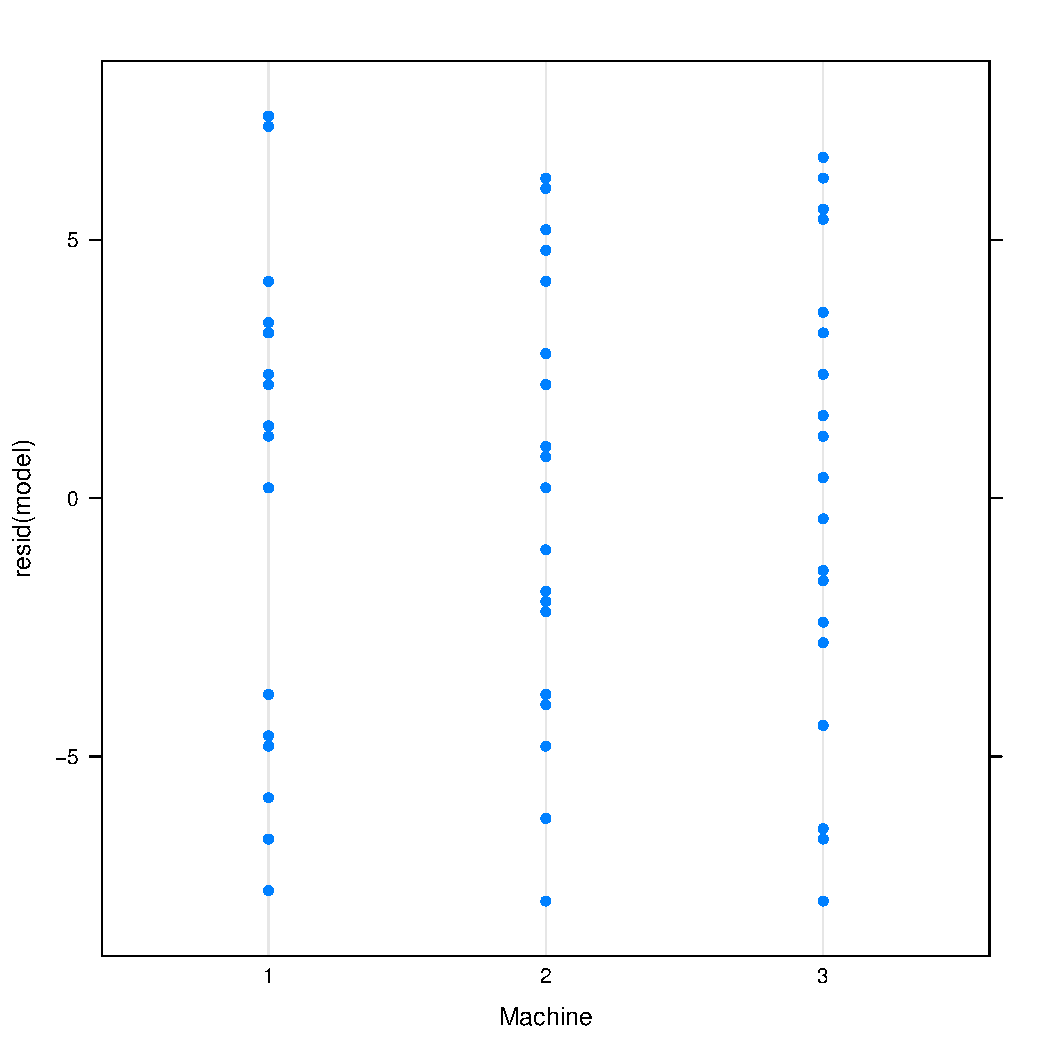
\includegraphics[width=\maxwidth]{figure/unnamed-chunk-2-1} 

\end{knitrout}

\qquad The plot shows no sign for unequal variance, so it support the assumption of constancy of the error variance.

\end{enumerate}

\section{26.5}

\begin{enumerate}[(a)]

\item
  
\qquad No.

\item

\begin{knitrout}
\definecolor{shadecolor}{rgb}{0.969, 0.969, 0.969}\color{fgcolor}\begin{kframe}
\begin{alltt}
  \hlkwd{dotplot}\hlstd{(dat}\hlopt{$}\hlstd{A} \hlopt{~} \hlstd{dat}\hlopt{$}\hlstd{Y,} \hlkwc{groups} \hlstd{= dat}\hlopt{$}\hlstd{B)}
\end{alltt}
\end{kframe}
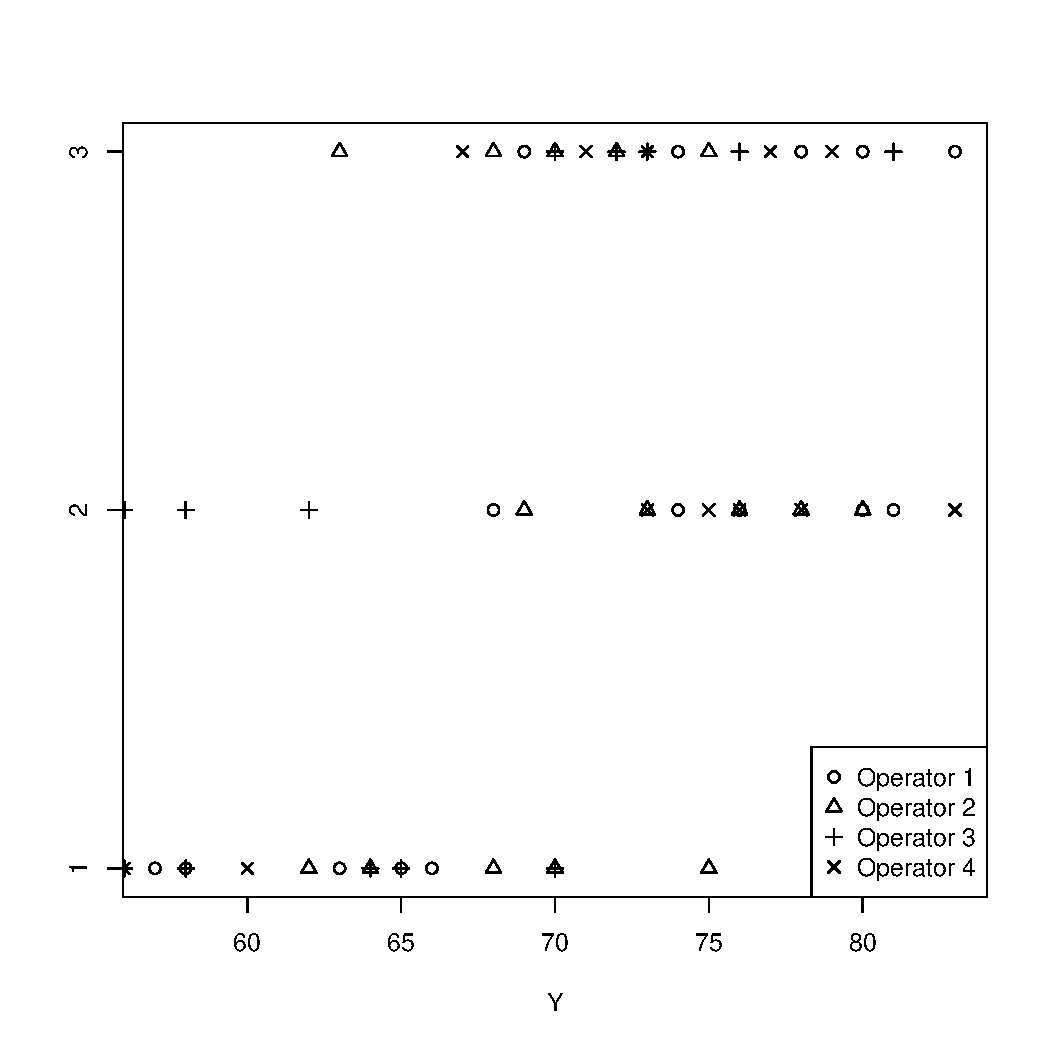
\includegraphics[width=\maxwidth]{figure/unnamed-chunk-3-1} 

\end{knitrout}

\qquad It seems operator effect are present.

\item

\begin{knitrout}
\definecolor{shadecolor}{rgb}{0.969, 0.969, 0.969}\color{fgcolor}\begin{kframe}
\begin{alltt}
  \hlkwd{summary}\hlstd{(model)}
\end{alltt}
\begin{verbatim}
##             Df Sum Sq Mean Sq F value   Pr(>F)    
## A            2   1696   847.8   35.92 2.90e-10 ***
## A:B          9   2272   252.5   10.70 6.99e-09 ***
## Residuals   48   1133    23.6                     
## ---
## Signif. codes:  0 '***' 0.001 '**' 0.01 '*' 0.05 '.' 0.1 ' ' 1
\end{verbatim}
\end{kframe}
\end{knitrout}

Test the mean outputs differ for three machine:

\begin{center}
$H_0$:all $\alpha_i$ equal zero(i=1,2,3)

VS. $H_1$:not all $\alpha_i$ equal zero

$F^*=\frac{MSA}{MSE} = 847.8/23.6  = 35.92$

we can reject $H_0$ if $F^* > F(1-0.01;2,48)=5.076664$,otherwise reject$H_1$

so that reject $H_0$ because $F^*>5.076664$,

therefore, the mean outputs differ for three machine, and the P-value is 2.90e-10
\end{center}

\item

Test the mean outputs differ for the operator:

\begin{center}
$H_0$:all $\beta_{j(i)}$ equal zero(i=1,2,3)

VS. $H_1$:not all $\beta_{j(i)}$ equal zero

$F^*=\frac{MSB(A)}{MSE} = 252.5/23.6  = 10.7$

we can reject $H_0$ if $F^* > F(1-0.01;9,48)=2.801816$,otherwise reject$H_1$

so that reject $H_0$ because $F^*>2.801816$,

therefore, our conclusion implies that operator within at least one machine differ in terms of mean shifts effects, and the P-value is 6.99e-09
\end{center}

\item

\begin{knitrout}
\definecolor{shadecolor}{rgb}{0.969, 0.969, 0.969}\color{fgcolor}\begin{kframe}
\begin{alltt}
  \hlstd{model1} \hlkwb{=} \hlkwd{aov}\hlstd{(Y} \hlopt{~} \hlstd{A} \hlopt{+} \hlstd{A}\hlopt{/}\hlstd{B,} \hlkwc{data} \hlstd{= dat)}
\end{alltt}
\end{kframe}
\end{knitrout}

\begin{center}
$H_0$:all $\beta_{j(i)}$ equal zero(i=1,2,3)

VS. $H_1$:not all $\beta_{j(i)}$ equal zero

$F^*=\frac{MSB(A)}{MSE} = 252.5/23.6  = 10.7$

we can reject $H_0$ if $F^* > F(1-0.01;9,48)=2.801816$,otherwise reject$H_1$

so that reject $H_0$ because $F^*>2.801816$,

therefore, our conclusion implies that operator within at least one machine differ in terms of mean shifts effects, and the P-value is 6.99e-09
\end{center}

\begin{center}
$H_0$:all $\beta_{j(i)}$ equal zero(i=1,2,3)

VS. $H_1$:not all $\beta_{j(i)}$ equal zero

$F^*=\frac{MSB(A)}{MSE} = 252.5/23.6  = 10.7$

we can reject $H_0$ if $F^* > F(1-0.01;9,48)=2.801816$,otherwise reject$H_1$

so that reject $H_0$ because $F^*>2.801816$,

therefore, our conclusion implies that operator within at least one machine differ in terms of mean shifts effects, and the P-value is 6.99e-09
\end{center}

\begin{center}
$H_0$:all $\beta_{j(i)}$ equal zero(i=1,2,3)

VS. $H_1$:not all $\beta_{j(i)}$ equal zero

$F^*=\frac{MSB(A)}{MSE} = 252.5/23.6  = 10.7$

we can reject $H_0$ if $F^* > F(1-0.01;9,48)=2.801816$,otherwise reject$H_1$

so that reject $H_0$ because $F^*>2.801816$,

therefore, our conclusion implies that operator within at least one machine differ in terms of mean shifts effects, and the P-value is 6.99e-09
\end{center}

\item

\begin{displaymath}
\begin{split}
  \alpha &\leq 1 -(1-\alpha_1)...(1-\alpha_5)\\
         &= 1-(1-0.05)^5\\
         &= 0.2262191
\end{split}
\end{displaymath}

\qquad We conclude that three machine differ in mean output, 4 operators in machine 1 have different mean output effect, 4 operators in machine 2 have different mean output effect, but 4 operators in machine 3 do not have different mean output effect.

\end{enumerate}

\section{26.6}

\begin{enumerate}[(a)]

\item

\begin{knitrout}
\definecolor{shadecolor}{rgb}{0.969, 0.969, 0.969}\color{fgcolor}\begin{kframe}
\begin{alltt}
  \hlstd{means} \hlkwb{=} \hlkwd{with}\hlstd{(dat,} \hlkwd{by}\hlstd{(Y, A, mean))}
  \hlstd{D1} \hlkwb{=} \hlstd{means[}\hlnum{1}\hlstd{]} \hlopt{-} \hlstd{means[}\hlnum{2}\hlstd{]}
  \hlstd{D2} \hlkwb{=} \hlstd{means[}\hlnum{1}\hlstd{]} \hlopt{-} \hlstd{means[}\hlnum{3}\hlstd{]}
  \hlstd{D3} \hlkwb{=} \hlstd{means[}\hlnum{2}\hlstd{]} \hlopt{-} \hlstd{means[}\hlnum{3}\hlstd{]}
  \hlstd{tukey} \hlkwb{=} \hlnum{1}\hlopt{/}\hlkwd{sqrt}\hlstd{(}\hlnum{2}\hlstd{)}\hlopt{*}\hlkwd{qtukey}\hlstd{(}\hlnum{0.95}\hlstd{,} \hlnum{3}\hlstd{,} \hlnum{48}\hlstd{)}
  \hlstd{tukey}
\end{alltt}
\begin{verbatim}
## [1] 2.418488
\end{verbatim}
\begin{alltt}
  \hlstd{mse} \hlkwb{=} \hlnum{23.6}
  \hlstd{s} \hlkwb{=} \hlkwd{sqrt}\hlstd{(}\hlnum{2}\hlopt{*}\hlstd{mse}\hlopt{/}\hlstd{(b}\hlopt{*}\hlstd{n))}
  \hlstd{s}
\end{alltt}
\begin{verbatim}
## [1] 1.536229
\end{verbatim}
\begin{alltt}
  \hlkwd{c}\hlstd{(D1}\hlopt{-}\hlstd{s}\hlopt{*}\hlstd{tukey, D1}\hlopt{+}\hlstd{s}\hlopt{*}\hlstd{tukey)}
\end{alltt}
\begin{verbatim}
##          1          1 
## -13.465351  -6.034649
\end{verbatim}
\begin{alltt}
  \hlkwd{c}\hlstd{(D2}\hlopt{-}\hlstd{s}\hlopt{*}\hlstd{tukey, D2}\hlopt{+}\hlstd{s}\hlopt{*}\hlstd{tukey)}
\end{alltt}
\begin{verbatim}
##          1          1 
## -16.065351  -8.634649
\end{verbatim}
\begin{alltt}
  \hlkwd{c}\hlstd{(D3}\hlopt{-}\hlstd{s}\hlopt{*}\hlstd{tukey, D3}\hlopt{+}\hlstd{s}\hlopt{*}\hlstd{tukey)}
\end{alltt}
\begin{verbatim}
##         2         2 
## -6.315351  1.115351
\end{verbatim}
\end{kframe}
\end{knitrout}

\begin{displaymath}
\begin{split}
\bar{Y}_{1\cdot \cdot} = 61.2 &, \bar{Y}_{2\cdot \cdot} = 70.95 , \bar{Y}_{3\cdot \cdot} = 73.55 \\
\hat{D}_1 = \bar{Y}_{1\cdot \cdot}-\bar{Y}_{2\cdot \cdot} = -9.75 &,  \hat{D}_2 = \bar{Y}_{1\cdot \cdot}-\bar{Y}_{3\cdot \cdot}=-12.35 , \hat{D}_3 = \bar{Y}_{2\cdot \cdot}-\bar{Y}_{3\cdot \cdot}=-2.6 \\
S = \sqrt{\frac{MSE}{bn}*2} = 1.536229 &, Tukey = \frac{1}{\sqrt{2}}\text{qtukey}(1-alpha, a, ab(n-1))=2.418488\\
\text{base on} &\hat{D}_i \pm S*T\\
-13.465351 & \leq D_1 \leq -6.034649  \\
-16.065351 &\leq D_2 \leq -8.634649 \\
-6.315351 &\leq D_3 \leq 1.115351  \\
\end{split}
\end{displaymath}

\qquad We conclude that with 95\% family confidence that the mean output is highest in machine 3, and the difference between machine 2 and machine 3 is not statistically significant.

\item

\begin{knitrout}
\definecolor{shadecolor}{rgb}{0.969, 0.969, 0.969}\color{fgcolor}\begin{kframe}
\begin{alltt}
  \hlstd{means} \hlkwb{=} \hlkwd{with}\hlstd{(dat,} \hlkwd{by}\hlstd{(Y,} \hlkwd{list}\hlstd{(A,B) , mean))}
  \hlstd{D1} \hlkwb{=} \hlstd{means[}\hlnum{1}\hlstd{,}\hlnum{1}\hlstd{]} \hlopt{-} \hlstd{means[}\hlnum{1}\hlstd{,}\hlnum{2}\hlstd{]}
  \hlstd{D2} \hlkwb{=} \hlstd{means[}\hlnum{1}\hlstd{,}\hlnum{1}\hlstd{]} \hlopt{-} \hlstd{means[}\hlnum{1}\hlstd{,}\hlnum{3}\hlstd{]}
  \hlstd{D3} \hlkwb{=} \hlstd{means[}\hlnum{1}\hlstd{,}\hlnum{1}\hlstd{]} \hlopt{-} \hlstd{means[}\hlnum{1}\hlstd{,}\hlnum{4}\hlstd{]}
  \hlstd{D4} \hlkwb{=} \hlstd{means[}\hlnum{1}\hlstd{,}\hlnum{2}\hlstd{]} \hlopt{-} \hlstd{means[}\hlnum{1}\hlstd{,}\hlnum{3}\hlstd{]}
  \hlstd{D5} \hlkwb{=} \hlstd{means[}\hlnum{1}\hlstd{,}\hlnum{2}\hlstd{]} \hlopt{-} \hlstd{means[}\hlnum{1}\hlstd{,}\hlnum{4}\hlstd{]}
  \hlstd{D6} \hlkwb{=} \hlstd{means[}\hlnum{1}\hlstd{,}\hlnum{3}\hlstd{]} \hlopt{-} \hlstd{means[}\hlnum{1}\hlstd{,}\hlnum{4}\hlstd{]}
  \hlstd{B} \hlkwb{=} \hlkwd{qt}\hlstd{(}\hlnum{1}\hlopt{-}\hlnum{0.05}\hlopt{/}\hlstd{(}\hlnum{2}\hlopt{*}\hlnum{6}\hlstd{), (n}\hlopt{-}\hlnum{1}\hlstd{)}\hlopt{*}\hlstd{a}\hlopt{*}\hlstd{b)}
  \hlstd{B}
\end{alltt}
\begin{verbatim}
## [1] 2.752023
\end{verbatim}
\begin{alltt}
  \hlstd{mse} \hlkwb{=} \hlnum{23.6}
  \hlstd{s} \hlkwb{=} \hlkwd{sqrt}\hlstd{(}\hlnum{2}\hlopt{*}\hlstd{mse}\hlopt{/}\hlstd{(n))}
  \hlstd{s}
\end{alltt}
\begin{verbatim}
## [1] 3.072458
\end{verbatim}
\begin{alltt}
  \hlkwd{c}\hlstd{(D1}\hlopt{-}\hlstd{s}\hlopt{*}\hlstd{B, D1}\hlopt{+}\hlstd{s}\hlopt{*}\hlstd{B)}
\end{alltt}
\begin{verbatim}
## [1] -14.455477   2.455477
\end{verbatim}
\begin{alltt}
  \hlkwd{c}\hlstd{(D2}\hlopt{-}\hlstd{s}\hlopt{*}\hlstd{B, D2}\hlopt{+}\hlstd{s}\hlopt{*}\hlstd{B)}
\end{alltt}
\begin{verbatim}
## [1] -9.255477  7.655477
\end{verbatim}
\begin{alltt}
  \hlkwd{c}\hlstd{(D3}\hlopt{-}\hlstd{s}\hlopt{*}\hlstd{B, D3}\hlopt{+}\hlstd{s}\hlopt{*}\hlstd{B)}
\end{alltt}
\begin{verbatim}
## [1]  0.7445233 17.6554767
\end{verbatim}
\begin{alltt}
  \hlkwd{c}\hlstd{(D4}\hlopt{-}\hlstd{s}\hlopt{*}\hlstd{B, D4}\hlopt{+}\hlstd{s}\hlopt{*}\hlstd{B)}
\end{alltt}
\begin{verbatim}
## [1] -3.255477 13.655477
\end{verbatim}
\begin{alltt}
  \hlkwd{c}\hlstd{(D5}\hlopt{-}\hlstd{s}\hlopt{*}\hlstd{B, D5}\hlopt{+}\hlstd{s}\hlopt{*}\hlstd{B)}
\end{alltt}
\begin{verbatim}
## [1]  6.744523 23.655477
\end{verbatim}
\begin{alltt}
  \hlkwd{c}\hlstd{(D6}\hlopt{-}\hlstd{s}\hlopt{*}\hlstd{B, D6}\hlopt{+}\hlstd{s}\hlopt{*}\hlstd{B)}
\end{alltt}
\begin{verbatim}
## [1]  1.544523 18.455477
\end{verbatim}
\end{kframe}
\end{knitrout}

\begin{displaymath}
\begin{split}
\bar{Y}_{11 \cdot} = 61.8 &, \bar{Y}_{12 \cdot} = 67.8 , \bar{Y}_{13 \cdot} = 62.6, \bar{Y}_{14 \cdot} = 52.6 \\
\hat{D}_1 = \bar{Y}_{11 \cdot}-\bar{Y}_{12 \cdot} = -6 &,  \hat{D}_2 = \bar{Y}_{11 \cdot}-\bar{Y}_{13 \cdot}=-0.8 , \hat{D}_3 = \bar{Y}_{11 \cdot}-\bar{Y}_{14 \cdot}=-9.2 \\
\hat{D}_4 = \bar{Y}_{12 \cdot}-\bar{Y}_{13 \cdot} =5.2 &,  \hat{D}_5 = \bar{Y}_{12 \cdot}-\bar{Y}_{14 \cdot}=15.2 , \hat{D}_6 = \bar{Y}_{13 \cdot}-\bar{Y}_{14 \cdot}=10 \\
S = \sqrt{\frac{MSE}{n}*2} = 3.072458 &, B = t(1-\alpha/(2*6), ab(n-1))=2.752023\\
\text{base on} &\hat{D}_i \pm S*B\\
-14.455477 & \leq D_1 \leq 2.455477  \\
-9.255477 &\leq D_2 \leq 7.655477 \\
0.7445233 &\leq D_3 \leq 17.6554767  \\
-3.255477 & \leq D_4 \leq 13.655477  \\
6.744523 &\leq D_5 \leq 23.655477\\
1.544523 &\leq D_6 \leq 18.455477  \\
\end{split}
\end{displaymath}

\qquad We conclude that with 95\% family confidence in machine 1 the differences between operator 1 and operator 2, operator 1 and operator 3, operator 2 and operator 3 are not statistically significant.

\item

\begin{knitrout}
\definecolor{shadecolor}{rgb}{0.969, 0.969, 0.969}\color{fgcolor}\begin{kframe}
\begin{alltt}
  \hlstd{L_hat} \hlkwb{=} \hlstd{(means[}\hlnum{1}\hlstd{,}\hlnum{1}\hlstd{]}\hlopt{+}\hlstd{means[}\hlnum{1}\hlstd{,}\hlnum{2}\hlstd{]}\hlopt{+}\hlstd{means[}\hlnum{1}\hlstd{,}\hlnum{3}\hlstd{])}\hlopt{/}\hlnum{3} \hlopt{-} \hlstd{means[}\hlnum{1}\hlstd{,}\hlnum{4}\hlstd{]}
  \hlstd{s} \hlkwb{=} \hlkwd{sqrt}\hlstd{(mse}\hlopt{/}\hlstd{(n)}\hlopt{*}\hlstd{((}\hlnum{1}\hlopt{/}\hlnum{3}\hlstd{)}\hlopt{^}\hlnum{2}\hlopt{*}\hlnum{3}\hlopt{+}\hlnum{1}\hlstd{))}
  \hlstd{s}
\end{alltt}
\begin{verbatim}
## [1] 2.508652
\end{verbatim}
\begin{alltt}
  \hlstd{t} \hlkwb{=} \hlkwd{qt}\hlstd{(}\hlnum{1}\hlopt{-}\hlnum{0.01}\hlopt{/}\hlnum{2}\hlstd{, a}\hlopt{*}\hlstd{b}\hlopt{*}\hlstd{(n}\hlopt{-}\hlnum{1}\hlstd{))}
  \hlstd{t}
\end{alltt}
\begin{verbatim}
## [1] 2.682204
\end{verbatim}
\begin{alltt}
  \hlkwd{c}\hlstd{(L_hat}\hlopt{-}\hlstd{s}\hlopt{*}\hlstd{t, L_hat}\hlopt{+}\hlstd{s}\hlopt{*}\hlstd{t)}
\end{alltt}
\begin{verbatim}
## [1]  4.737951 18.195382
\end{verbatim}
\end{kframe}
\end{knitrout}

\begin{displaymath}
\begin{split}
\hat{L} &= \frac{\bar{Y}_{11\cdot}+\bar{Y}_{12\cdot}+\bar{Y}_{13\cdot}}{3}+\bar{Y}_{14\cdot} = 11.46667\\
c_1 &= c_2 = c_3 = 1/3, c_4 = -1\\
S &= \sqrt{\frac{MSE}{n}*\sum_i c_i^2} = 2.508652 \\
t &= t(1-\alpha/2, ab(n-1))=2.682204\\
\text{base on } &\hat{L} \pm S*t\\
4.737951 & \leq D_1 \leq 18.195382  \\
\end{split}
\end{displaymath}

\qquad We are 99\% confident that L is between 0.737951 and  18.195382.

\end{enumerate}

\section{26.7}

\begin{enumerate}[(a)]

\item

\qquad $\beta_{j(i)}$ are $i.i.d$ $N(0, \sigma^2_\beta$, and $\beta_{j(i)}$ and $\epsilon_{ijk}$ are independent.

\item

\begin{knitrout}
\definecolor{shadecolor}{rgb}{0.969, 0.969, 0.969}\color{fgcolor}\begin{kframe}
\begin{alltt}
  \hlstd{model_new} \hlkwb{=} \hlkwd{aov}\hlstd{(Y} \hlopt{~} \hlstd{A}\hlopt{+} \hlkwd{Error}\hlstd{(A}\hlopt{/}\hlstd{B),} \hlkwc{data} \hlstd{= dat)}
  \hlkwd{summary}\hlstd{(model_new)}
\end{alltt}
\begin{verbatim}
## 
## Error: A
##   Df Sum Sq Mean Sq
## A  2   1696   847.8
## 
## Error: A:B
##           Df Sum Sq Mean Sq F value Pr(>F)
## Residuals  9   2272   252.5               
## 
## Error: Within
##           Df Sum Sq Mean Sq F value Pr(>F)
## Residuals 48   1133    23.6
\end{verbatim}
\begin{alltt}
  \hlstd{s_square} \hlkwb{=} \hlstd{(}\hlnum{252.5}\hlopt{-}\hlnum{23.6}\hlstd{)}\hlopt{/}\hlstd{n}
  \hlstd{s_square}
\end{alltt}
\begin{verbatim}
## [1] 45.78
\end{verbatim}
\end{kframe}
\end{knitrout}

\begin{displaymath}
\begin{split}
E(MSB(A)) &= \sigma^2 + n\sigma^2_{\beta}\\
E(MSE) &= \sigma^2 \\
\hat{\sigma}_\beta^2 &= s^2_\beta = (MSB(A)-MSE)/n = 45.78
\end{split}
\end{displaymath}

\item

Test:

\begin{center}
$H_0$:$\sigma^2_\beta = 0$

VS. $H_1$:$\sigma^2_\beta \ne 0$

$F^*=\frac{MSB(A)}{MSE} = 252.5/23.6  = 10.7$

we can reject $H_0$ if $F^* > F(1-0.01;9,48)=1.765318$,otherwise reject$H_1$

so that reject $H_0$ because $F^*>1.765318$,

therefore, our conclusion implies that operator within at least one machine differ in terms of mean shifts effects, and the P-value is 6.976208e-09
\end{center}

\begin{knitrout}
\definecolor{shadecolor}{rgb}{0.969, 0.969, 0.969}\color{fgcolor}\begin{kframe}
\begin{alltt}
  \hlstd{c1}\hlkwb{=}\hlnum{1}\hlopt{/}\hlnum{5}
  \hlstd{c2}\hlkwb{=}\hlopt{-}\hlnum{1}\hlopt{/}\hlnum{5}
  \hlstd{ms1}\hlkwb{=}\hlnum{252.5}
  \hlstd{ms2}\hlkwb{=}\hlnum{23.6}
  \hlstd{df1}\hlkwb{=}\hlnum{9}
  \hlstd{df2}\hlkwb{=}\hlnum{48}
  \hlstd{F1}\hlkwb{=}\hlkwd{qf}\hlstd{(}\hlnum{.95}\hlstd{,df1,}\hlnum{Inf}\hlstd{)}
  \hlstd{F2}\hlkwb{=}\hlkwd{qf}\hlstd{(}\hlnum{.95}\hlstd{,df2,}\hlnum{Inf}\hlstd{)}
  \hlstd{F3}\hlkwb{=}\hlkwd{qf}\hlstd{(}\hlnum{.95}\hlstd{,}\hlnum{Inf}\hlstd{,df1)}
  \hlstd{F4}\hlkwb{=}\hlkwd{qf}\hlstd{(}\hlnum{.95}\hlstd{,}\hlnum{Inf}\hlstd{,df2)}
  \hlstd{F5}\hlkwb{=}\hlkwd{qf}\hlstd{(}\hlnum{.95}\hlstd{,df1,df2)}
  \hlstd{F6}\hlkwb{=}\hlkwd{qf}\hlstd{(}\hlnum{.95}\hlstd{,df2,df1)}
  \hlstd{G1}\hlkwb{=}\hlnum{1}\hlopt{-}\hlnum{1}\hlopt{/}\hlstd{F1}
  \hlstd{G2}\hlkwb{=}\hlnum{1}\hlopt{-}\hlnum{1}\hlopt{/}\hlstd{F2}
  \hlstd{G3}\hlkwb{=}\hlstd{((F5}\hlopt{-}\hlnum{1}\hlstd{)}\hlopt{^}\hlnum{2}\hlopt{-}\hlstd{(G1}\hlopt{*}\hlstd{F5)}\hlopt{^}\hlnum{2}\hlopt{-}\hlstd{(F4}\hlopt{-}\hlnum{1}\hlstd{)}\hlopt{^}\hlnum{2}\hlstd{)}\hlopt{/}\hlstd{F5}
  \hlstd{G4}\hlkwb{=}\hlstd{F6}\hlopt{*}\hlstd{( ((F6}\hlopt{-}\hlnum{1}\hlstd{)}\hlopt{/}\hlstd{F6)}\hlopt{^}\hlnum{2} \hlopt{-} \hlstd{((F3}\hlopt{-}\hlnum{1}\hlstd{)}\hlopt{/}\hlstd{F6)}\hlopt{^}\hlnum{2} \hlopt{-} \hlstd{G2}\hlopt{^}\hlnum{2} \hlstd{)}
  \hlstd{Hl} \hlkwb{=} \hlkwd{sqrt}\hlstd{( (G1}\hlopt{*}\hlstd{c1}\hlopt{*}\hlstd{ms1)}\hlopt{^}\hlnum{2} \hlopt{+} \hlstd{((F4}\hlopt{-}\hlnum{1}\hlstd{)}\hlopt{*}\hlstd{c2}\hlopt{*}\hlstd{ms2)}\hlopt{^}\hlnum{2} \hlopt{-} \hlstd{G3}\hlopt{*}\hlstd{c1}\hlopt{*}\hlstd{c2}\hlopt{*}\hlstd{ms1}\hlopt{*}\hlstd{ms2)}
  \hlstd{Hl}
\end{alltt}
\begin{verbatim}
## [1] 23.77552
\end{verbatim}
\begin{alltt}
  \hlstd{Hu} \hlkwb{=} \hlkwd{sqrt}\hlstd{( (G2}\hlopt{*}\hlstd{c2}\hlopt{*}\hlstd{ms2)}\hlopt{^}\hlnum{2} \hlopt{+} \hlstd{((F3}\hlopt{-}\hlnum{1}\hlstd{)}\hlopt{*}\hlstd{c1}\hlopt{*}\hlstd{ms1)}\hlopt{^}\hlnum{2} \hlopt{-} \hlstd{G4}\hlopt{*}\hlstd{c1}\hlopt{*}\hlstd{c2}\hlopt{*}\hlstd{ms1}\hlopt{*}\hlstd{ms2)}
  \hlstd{Hu}
\end{alltt}
\begin{verbatim}
## [1] 86.09976
\end{verbatim}
\begin{alltt}
  \hlstd{sigma_mu} \hlkwb{=}  \hlstd{(ms1}\hlopt{-}\hlstd{ms2)}\hlopt{/}\hlstd{(n)}
  \hlkwd{c}\hlstd{(}\hlkwd{max}\hlstd{(}\hlnum{0}\hlstd{,sigma_mu}\hlopt{-}\hlstd{Hl), sigma_mu}\hlopt{+}\hlstd{Hu)}
\end{alltt}
\begin{verbatim}
## [1]  22.00448 131.87976
\end{verbatim}
\end{kframe}
\end{knitrout}

\begin{center}
E(MSB(A))= $nb\sigma_\beta^2+\sigma^2$ \qquad E(MSE)=$\sigma^2$\\
Base on $L=\sigma_\mu^2=c_1E(MSB(A))+c_2E(MSE)$\\
then $c_1=1/(n)=0.2$, $c_2=-1/(n)=-0.2$\\
and $MSB(A)=252.5, MSE=23.6, df1=9, df2=48$\\
\end{center}

According to MLS procedure, $H_l=22.00448$ \qquad $H_u=131.87976$ \qquad $\sigma_\beta^2=45.78$

\qquad so that 90\% confident interval is  $s^2_\beta-H_l \leq \sigma_\mu^2 \leq s^2_\beta+H_u$,which means $22.00448 \leq \sigma_\beta^2 \leq 131.87976$

\item

Test the mean outputs differ for three machine:

\begin{center}
$H_0$:all $\alpha_i$ equal zero(i=1,2,3)

VS. $H_1$:not all $\alpha_i$ equal zero

$F^*=\frac{MSA}{MSB(A)} = 847.8/252.5  = 3.357624$

we can reject $H_0$ if $F^* > F(1-0.1;2,9)=3.006452$,otherwise reject$H_1$

so that reject $H_0$ because $F^*>3.006452$,

therefore, the mean outputs differ for three machine, and the P-value is 0.08140399
\end{center}

\item

\begin{knitrout}
\definecolor{shadecolor}{rgb}{0.969, 0.969, 0.969}\color{fgcolor}\begin{kframe}
\begin{alltt}
  \hlstd{means} \hlkwb{=} \hlkwd{with}\hlstd{(dat,} \hlkwd{by}\hlstd{(Y, A, mean))}
  \hlstd{D1} \hlkwb{=} \hlstd{means[}\hlnum{1}\hlstd{]} \hlopt{-} \hlstd{means[}\hlnum{2}\hlstd{]}
  \hlstd{D2} \hlkwb{=} \hlstd{means[}\hlnum{1}\hlstd{]} \hlopt{-} \hlstd{means[}\hlnum{3}\hlstd{]}
  \hlstd{D3} \hlkwb{=} \hlstd{means[}\hlnum{2}\hlstd{]} \hlopt{-} \hlstd{means[}\hlnum{3}\hlstd{]}
  \hlstd{tukey} \hlkwb{=} \hlnum{1}\hlopt{/}\hlkwd{sqrt}\hlstd{(}\hlnum{2}\hlstd{)}\hlopt{*}\hlkwd{qtukey}\hlstd{(}\hlnum{0.9}\hlstd{,} \hlnum{3}\hlstd{,} \hlnum{9}\hlstd{)}
  \hlstd{tukey}
\end{alltt}
\begin{verbatim}
## [1] 2.344595
\end{verbatim}
\begin{alltt}
  \hlstd{msb_a} \hlkwb{=} \hlnum{252.5}
  \hlstd{s} \hlkwb{=} \hlkwd{sqrt}\hlstd{(}\hlnum{2}\hlopt{*}\hlstd{msb_a}\hlopt{/}\hlstd{(b}\hlopt{*}\hlstd{n))}
  \hlstd{s}
\end{alltt}
\begin{verbatim}
## [1] 5.024938
\end{verbatim}
\begin{alltt}
  \hlkwd{c}\hlstd{(D1}\hlopt{-}\hlstd{s}\hlopt{*}\hlstd{tukey, D1}\hlopt{+}\hlstd{s}\hlopt{*}\hlstd{tukey)}
\end{alltt}
\begin{verbatim}
##          1          1 
## -21.531444   2.031444
\end{verbatim}
\begin{alltt}
  \hlkwd{c}\hlstd{(D2}\hlopt{-}\hlstd{s}\hlopt{*}\hlstd{tukey, D2}\hlopt{+}\hlstd{s}\hlopt{*}\hlstd{tukey)}
\end{alltt}
\begin{verbatim}
##          1          1 
## -24.131444  -0.568556
\end{verbatim}
\begin{alltt}
  \hlkwd{c}\hlstd{(D3}\hlopt{-}\hlstd{s}\hlopt{*}\hlstd{tukey, D3}\hlopt{+}\hlstd{s}\hlopt{*}\hlstd{tukey)}
\end{alltt}
\begin{verbatim}
##          2          2 
## -14.381444   9.181444
\end{verbatim}
\end{kframe}
\end{knitrout}

\begin{displaymath}
\begin{split}
\bar{Y}_{1\cdot \cdot} = 61.2 &, \bar{Y}_{2\cdot \cdot} = 70.95 , \bar{Y}_{3\cdot \cdot} = 73.55 \\
\hat{D}_1 = \bar{Y}_{1\cdot \cdot}-\bar{Y}_{2\cdot \cdot} = -9.75 &,  \hat{D}_2 = \bar{Y}_{1\cdot \cdot}-\bar{Y}_{3\cdot \cdot}=-12.35 , \hat{D}_3 = \bar{Y}_{2\cdot \cdot}-\bar{Y}_{3\cdot \cdot}=-2.6 \\
S = \sqrt{\frac{MSB(A)}{bn}*2} = 5.024938 &, Tukey = \frac{1}{\sqrt{2}}\text{qtukey}(1-alpha, a, a(b-1)=2.344595\\
\text{base on} &\hat{D}_i \pm S*T\\
-21.531444 & \leq D_1 \leq 2.031444   \\
-24.131444 &\leq D_2 \leq -0.568556 \\
-14.381444 &\leq D_3 \leq 9.181444   \\
\end{split}
\end{displaymath}

\qquad We conclude that with 95\% family confidence that the mean output is highest in machine 3, and the differences between machine 2 and machine 3, machine 1 and machine 2 are not statistically significant.

\item

\begin{knitrout}
\definecolor{shadecolor}{rgb}{0.969, 0.969, 0.969}\color{fgcolor}\begin{kframe}
\begin{alltt}
  \hlstd{dat_reg} \hlkwb{=} \hlstd{dat}
  \hlstd{med1} \hlkwb{=} \hlkwd{median}\hlstd{(dat_reg}\hlopt{$}\hlstd{Y[dat_reg}\hlopt{$}\hlstd{A}\hlopt{==}\hlnum{1}\hlstd{])}
  \hlstd{med2} \hlkwb{=} \hlkwd{median}\hlstd{(dat_reg}\hlopt{$}\hlstd{Y[dat_reg}\hlopt{$}\hlstd{A}\hlopt{==}\hlnum{2}\hlstd{])}
  \hlstd{med3} \hlkwb{=} \hlkwd{median}\hlstd{(dat_reg}\hlopt{$}\hlstd{Y[dat_reg}\hlopt{$}\hlstd{A}\hlopt{==}\hlnum{3}\hlstd{])}
  \hlstd{d} \hlkwb{=} \hlkwd{abs}\hlstd{(dat_reg}\hlopt{$}\hlstd{Y} \hlopt{-} \hlkwd{c}\hlstd{(}\hlkwd{rep}\hlstd{(med1,}\hlnum{20}\hlstd{),}\hlkwd{rep}\hlstd{(med2,}\hlnum{20}\hlstd{),}\hlkwd{rep}\hlstd{(med3,}\hlnum{20}\hlstd{)))}
  \hlstd{model_fi} \hlkwb{=} \hlkwd{aov}\hlstd{(d} \hlopt{~} \hlkwd{factor}\hlstd{(dat_reg}\hlopt{$}\hlstd{A))}
  \hlkwd{summary}\hlstd{(model_fi)}
\end{alltt}
\begin{verbatim}
##                   Df Sum Sq Mean Sq F value Pr(>F)
## factor(dat_reg$A)  2    109   54.52   1.923  0.155
## Residuals         57   1616   28.35
\end{verbatim}
\end{kframe}
\end{knitrout}

Test:

Set $d_{ij} = | Y_{ij} - \tilde{Y}_i |$

\begin{center}
$H_0$:all $\sigma^2(\beta_{j(i)})$ are equal(i=1,2,3)

VS. $H_1$:not all $\sigma^2(\beta_{j(i)})$ are equal zero

$F^*_{BF}=\frac{MSTR(d)}{MSE(d)} = 109.85/34.02  = 3.228983$

we can reject $H_0$ if $F^* > F(1-0.01;2,9)=8.021517$,otherwise reject$H_1$

so that reject $H_1$ because $F^*<8.021517$,

therefore, all $\sigma^2(\beta_{j(i)})$ are equal(i=1,2,3)
\end{center}

\end{enumerate}

\section{26.19}

\section{26.20}

\section{26.24}

\begin{displaymath}
\begin{split}
SSB+SSAB &= na\sum_{j}(\bar{Y}_{\cdot j \cdot}-\bar{Y}_{\cdots})^2 + n\sum_i\sum_j(\bar{Y}_{ij\cdot}-\bar{Y}_{i\cdot\cdot}-\bar{Y}_{\cdot j \cdot}+\bar{Y}_{\cdots})^2
\end{split}
\end{displaymath}

\section{26.25}

\begin{enumerate}[(a)]

\item

Since

$$\bar{Y}_{ijk} = \mu_{ij} + \alpha_i + \beta_{j (i)} + \epsilon_{ijk}$$

then:

\begin{displaymath}
\begin{split}
\sigma^2 \{ \bar{Y}_{i\cdot\cdot} \} &= \sigma^2 \{ \mu_{i\cdot\cdot} + \alpha_i + \bar{\beta}_{\cdot (i)} + \bar{\epsilon}_{i\cdot\cdot} \} \\
                        &= \sigma^2 \{ \bar{\beta}_{\cdot (i)} + \bar{\epsilon}_{i\cdot\cdot} \} \\
                        &= \frac{\sigma^2_{\beta}}{b} + \frac{\sigma^2}{bn}  \qquad \text{,since $\beta$ and $\epsilon$ are independent}
\end{split}
\end{displaymath}

\begin{displaymath}
\begin{split}
\sigma^2 \{ \bar{Y}_{\cdot\cdot\cdot} \} &= \sigma^2 \{ \mu_{\cdot\cdot\cdot}  + \bar{\beta}_{\cdot (\cdot)} + \bar{\epsilon}_{\cdot\cdot\cdot} \} \qquad \text{,since $\sum_i \alpha=0$}\\
                        &= \sigma^2 \{ \bar{\beta}_{\cdot (\cdot)} + \bar{\epsilon}_{\cdot\cdot\cdot} \} \\
                        &= \frac{\sigma^2_{\beta}}{ab} + \frac{\sigma^2}{abn}  \qquad \text{,since $\beta$ and $\epsilon$ are independent}
\end{split}
\end{displaymath}

\item

\begin{displaymath}
\begin{split}
E(MSB(A)) &= \sigma^2 + n\sigma^2_{\beta}\\
E(MSE) &= \sigma^2 \\
s^2_\beta &= (MSB(A)-MSE)/n\\
\hat{\sigma}_\beta^2 &= max(0, s^2_\beta) = max(0, (MSB(A)-MSE)/n)
\end{split}
\end{displaymath}

\end{enumerate}

\section{26.28}



\end{document}
